%%%%%%%%%%%%%%%%%%%%%%%%%%%%%%%%%%%%%%%%%
% Journal Article
% LaTeX Template
% Version 1.3 (9/9/13)
%
% This template has been downloaded from:
% http://www.LaTeXTemplates.com
%
% Original author:
% Frits Wenneker (http://www.howtotex.com)
%
% License:
% CC BY-NC-SA 3.0 (http://creativecommons.org/licenses/by-nc-sa/3.0/)
%
%%%%%%%%%%%%%%%%%%%%%%%%%%%%%%%%%%%%%%%%%

%----------------------------------------------------------------------------------------
%	PACKAGES AND OTHER DOCUMENT CONFIGURATIONS
%----------------------------------------------------------------------------------------
\documentclass[twoside]{article}

\usepackage{mathtools}
\usepackage{amsmath}
\usepackage{algorithm}
\usepackage[noend]{algpseudocode}
\usepackage{amsthm}

\newtheorem{claim}{Claim} 

\usepackage{graphicx}
\graphicspath{ {figures/} }

\usepackage[usenames,dvipsnames]{color} % Required for specifying custom colors and referring to colors by name

\definecolor{MyRed}{rgb}{0.6, 0.0, 0.0} 
\definecolor{MyGreen}{rgb}{0.0,0.4,0.0} % Comment color
\definecolor{MyBlue}{rgb}{0.0, 0.0, 0.6}

%\setlength\parindent{24pt}

\usepackage[pdftex]{hyperref} % For hyperlinks in the PDF
\hypersetup{
  colorlinks=true,
  linkcolor=MyBlue, 
  citecolor=MyRed,
  urlcolor= MyGreen
}

% make hyperlinks bold
\newcommand{\aref}[1]
 {\textbf{\autoref{#1}}}

\newcommand{\nref}[1]
 {\textbf{\nameref{#1}}}

\newcommand{\cc}[1]
 {\textbf{\cite{#1}}}

\usepackage{lipsum} % Package to generate dummy text throughout this template

\usepackage[sc]{mathpazo} % Use the Palatino font
\usepackage[T1]{fontenc} % Use 8-bit encoding that has 256 glyphs
\linespread{1.05} % Line spacing - Palatino needs more space between lines
\usepackage{microtype} % Slightly tweak font spacing for aesthetics

\usepackage[hmarginratio=1:1,top=32mm,columnsep=20pt]{geometry} % Document margins
\usepackage{multicol} % Used for the two-column layout of the document
\usepackage[hang, small,labelfont=bf,up,textfont=it,up]{caption} % Custom captions under/above floats in tables or figures
\usepackage{booktabs} % Horizontal rules in tables
\usepackage{float} % Required for tables and figures in the multi-column environment - they need to be placed in specific locations with the [H] (e.g. \begin{table}[H])
\usepackage{hyperref} % For hyperlinks in the PDF

\usepackage{lettrine} % The lettrine is the first enlarged letter at the beginning of the text
\usepackage{paralist} % Used for the compactitem environment which makes bullet points with less space between them

\usepackage{abstract} % Allows abstract customization
\renewcommand{\abstractnamefont}{\normalfont\bfseries} % Set the "Abstract" text to bold
\renewcommand{\abstracttextfont}{\normalfont\small\itshape} % Set the abstract itself to small italic text

\usepackage{titlesec} % Allows customization of titles
%\renewcommand\thesection{\Roman{section}} % Roman numerals for the sections
%\renewcommand\thesubsection{\Roman{subsection}} % Roman numerals for subsections
\titleformat{\section}[block]{\large\scshape\centering}{\thesection.}{1em}{} % Change the look of the section titles
\titleformat{\subsection}[block]{\large}{\thesubsection.}{1em}{} % Change the look of the section titles


%----------------------------------------------------------------------------------------
%	TITLE SECTION
%----------------------------------------------------------------------------------------

\title{\vspace{-15mm}\fontsize{24pt}{10pt}\selectfont\textbf{Estimating Trending Topics on Twitter with Small Subsets of the Total Data}} % Article title

\author{
\large
\textsc{Evan Miller}\\[2mm] 
\textsc{Kiran Vodrahalli}\\[2mm]
\textsc{Albert Lee}\\[2mm]
\vspace{-5mm}
}
\date{January 13, 2015}

%----------------------------------------------------------------------------------------

\begin{document}

\maketitle % Insert title

%----------------------------------------------------------------------------------------
%	ABSTRACT
%----------------------------------------------------------------------------------------

\begin{abstract}

\noindent \lipsum[1] % Dummy abstract text

\end{abstract}

%----------------------------------------------------------------------------------------
%	ARTICLE CONTENTS
%----------------------------------------------------------------------------------------


\section{Introduction} \label{sec:Intro}

% introduction 
Since its founding in $2006$, Twitter has grown into a corporation dominating a significant
proporition of social media today. In recent years, it has become interesting to analyze tweets
to determine interesting phenomena ranging from the viral spread of news to the detection of earthquakes \cc{Burks:2014}. The volume of existing tweets is prohibitively large for standard methods of analysis, and requires approaches that are able to either store large amounts of data in memory for fast access (including parallel approaches to data processing) or approaches that only require sublinear memory while retaining accuracy guarantees. In this paper, we investigate a problem utilizing the latter method. 

\subsection{Problem Statement} 

% give clear definition of problem and motivation here
We would like to create an online algorithm that provides a real-time estimate of the frequencies of hashtags on Twitter time series data.
Since we want to be able to run this algorithm in real time, we would like for it to be space-efficient: that is, it should not be required to store a large number of hashtag counts at any given time. Ideally, the algorithm's space complexity should be sublinear in the number of hashtags seen. 
Therefore, our estimate should not require the exact frequency history of hashtags in tweets. 

More specifically, we will attempt to approximate the $k$ most popular Twitter hashtags in the time intervals of length $y$ in order to tell what is trending during that time period.
The idea is that estimating the top $k$ hashtags in some time interval provides a model for the topics that are trending on Twitter in that time period.


\subsection{Previous Work} \label{sec:PreviousWork}

% describe past work in the areas here

Some approaches attempt to do this by storing all of the frequency data, and looking at recent spikes while conditioning on all of the past frequency data in order to determine estimates of trending likelihood. We would like to improve the space complexity of this solution. Our approach will differ in that we will not store all the data of the past, but instead use several Count-Min Sketches to approximate the past frequencies. 

MIT people played with Tweet data to predict future trends \cc{MITNews2012}. 

As a preliminary starting point for approximating the past frequencies, we will utilize concepts from Matusevych et al.'s Hokusai paper to generalize the Count-Min Sketch scheme to time-series data \cc{Matusevych:2012}. The rough idea behind this approach is that in the distant past, we should only care about heavy-hitters, i.e. hashtags with high frequencies in order to estimate the likelihood that the hashtag is trending again.
% m is # hash, change it to d
% n is size of each hash, change it to m
The goal of the time-aggregated Hokusai system is to store older data at decreased precision since the older data also has decreased value in the computation.  The time-aggregated Hokusai system works by storing aggregate data in Count-Min sketches each with a $2^i$ day resolution for the past $2^i$ days.  Each of these Count-Min sketches computes $d$ hash functions from $\{0,1\}^*$ to $\{0, 1, ..., m-1\}$.


\subsection{Our Approaches}

why we don't use raw frequency counts for the past hour:
there are some hashtags that are constantly present (for example, $\#$porn, $\#$gamesinsight, $\#$teamfollowback (a way to get Twitter followers fast))
these should not be counted as 'trending', so we need to filter these out
with the history. what remains is 'what is trending'

Essentially, we must estimate a probability distribution for a finite set of labels in some moving time window of fixed size. Our labels will be Twitter hashtags, and we will take the window size to be 3 hours.

We will store the exact counts for the present (3 hour window), and continuously update the past and present as new data streams in. 

We had two different algorithms for finding out which hashtags were trending in real time, both space efficient.
The first algorithm, which we will describe as the naive algorithm, does not take into account the history and simply looks at the three hours before the current $3$-hour interval to find the current trending hashtags. We believe that in order to accurately determine trending hashtags, we will need to use more of the past in order to eliminate the hashtags which are ever-present, and therefore not trending. 


% not true, edit accordingly 
The baseline comparison for our performance will be the naive version of frequency tallying -- we will keep track of the entire history of frequencies, and will use the past to inform the present probability as to whether or not a given hashtag is trending. We also plan to provide a graphic of the top k hashtags, with histogram changing in real time as the estimated frequencies change. Regarding the data, we would ideally gain access to Twitter's firehose of tweets (as only a small subset of the true data is provided for those without access). 
%------------------------------------------------

\section{Describing the Algorithm}

% to note: our goal was to make a real time query algorithm that USES
% the history (in condensed form) to help understand current time 
% we're remembering the past with less accuracy to save space (realistic model)
% in order to get good estimates of present trending
% this means we are not trying to query the past the way Hokusai is.

% how did we approach it 
We separate the problem of finding trending topics on Twitter into two parts.  First, we need to maintain a data structure that efficiently stores data about all occurrences of every hashtag seen in the past.  We also maintain a separate data structure that allows us to quickly gather information about the most recent hashtags seen.

We want the former data structure to be very space efficient since it must store data about a very large dataset.  For this structure, space efficiency is more important than accuracy since small deviations in such a large dataset should not be significant because the deviations in past data should not greatly affect what is currently trending.

For the latter data structure, accuracy is more important than space efficiency since the structure contains data which more closely relates to which topics are currently trending and the size of the dataset is much smaller.


\subsection{Data Structures}
% -- we maintain datastructure in two parts: History, and Present
\subsubsection{History Data Structure}

To store data about all occurrences of every hashtag seen in the past, we use a modified version of the time-aggregated Hokusai system \cc{Matusevych:2012}, which is an extension of the Count-Min sketch. We previously described this data structure in \nref{sec:PreviousWork}. 
To the Hokusai structure we add another Count-Min sketch that combines the information from the Hokusai Count-Min sketches. We call this external Count-Min sketch the Kernel, since it acts as a weighting function on the CM sketches in the Hokusai structure. Its role is to depreciate the value of older data.
Denoting the CM sketches of the Hokusai structure as a vector $\textbf{M} = \{\overline{M}, M^0, M^1, ..., M^{{\lfloor {\log(T)} \rfloor}}\}$, where $\bar{M}$ is the Count-Min sketch storing the data of a unit time step (of size $z$), $M^j$ is the Count-Min sketch storing the data for the sketch with a $2^j$ time resolution, and $T$ is an upper bound on the number of $z$-units stored by the data structure. Then, the kernel function is given by

\begin{equation} 
\label{eq:kernel}
\textit{k}(\textbf{M}) = \overline{M} + \sum\limits_{j=0}^{{\lfloor \log⁡(T) \rfloor}} \frac{M^j}{2^j}
\end{equation}

For each hashtag, the kernel sketch stores a positive value between $0$ and $2$ (though typically $\leq 1$) that approximates how often the hashtag showed up in the past. In \nref{sec:Correctness} we will show that this aggregate Count-Min sketch weights the hashtags that occurred $i > 0$ days ago with weight approximately $\frac{1}{i}$.

We will refer to the combined data structure of Hokusai and the Kernel as the History.

\subsubsection{Current-Window Data Structure}

Our data structure for holding hashtags seen in the last $y$-length time period consists of three components: a max Fibonacci heap, a queue, and a hash table.  We refer to these components collectively as the Current Window.

The keys for the hash table are the hashtags, and the values stored in the table are (frequency, pointer to corresponding node in heap) pairs.

The queue contains (hashtag, timestamp) pairs, each of which is inserted upon seeing a hashtag in the input stream.

The heap has keys equal to (frequency in last $y$-length time period) / (value in Hokusai data structure) for a specific hashtag, and the value stored in the node is the corresponding hashtag.


\subsection{Algorithm Pseudocode} 

\subsubsection{Updating Hokusai data structure}

Algorithm \ref{alg1} describes the necessary steps to maintain the Hokusai data structure as new input is provided. We perform Time Aggregation. 

\begin{algorithm}
\caption{Update History} \label{alg1}
\begin{algorithmic}[1]
\ForAll {$i$}
	\State Initialize Count-Min sketch $M^i = 0$
\EndFor
\State Initialize $t = 0$
\State Initialize Count-Min sketches $\bar{M} = 0$ and $A = 0$
\While {data arrives}
	\State Aggregate data into sketch $\bar{M}$ for current $z$-unit while also adding this data to $A$
	\State $t \leftarrow t + 1$ (increment counter)
	\State $A \leftarrow A - \bar{M}$
	\For {$j = 0$ to argmax \{$l$ where $t$ mod $2^l = 0$\}}
		\State $A \leftarrow A + 2^{-j}(\bar{M} - M^j)$
		\State $T \leftarrow \bar{M}$ (back up temporary storage)
		\State $\bar{M} \leftarrow \bar{M} + M^j$ (increment cumulative sum)
		\State $M^j \leftarrow T$ (new value for $M^j$)
	\EndFor
	\State $\bar{M} \leftarrow 0$ (reset aggregator)
\EndWhile
\end{algorithmic}
\end{algorithm}
 


\subsubsection{Updating heap and hash tables}

This is 2.

\begin{algorithm}
\caption{Update Current-Window}\label{alg2}
\begin{algorithmic}[1]
\While {data arrives}
	\If {the current $z$-unit is different than that of the last hashtag seen}
		\State Do all the end-of-$z$ aggregation for the Hokusai structure as detailed in Algorithm \ref{alg1}.
		\ForAll {elements in the Fibonacci heap}
			\State look up the hashtag corresponding to this node in the hash table
			\State Update the key of the node to: \[\frac{\textnormal{frequency in last } y-\textnormal{length time period found at the table entry}}{\textnormal{new value in Hokusai data structure}}\]
		\EndFor
	\EndIf
	\If {queue is not empty}
		\State Peek at end of queue.
		\If {the timestamp + $y$ is before the current time}
			\State Look up the hashtag in the hash table and decrement the stored frequency.
			\If {the frequency is now 0}
				\State Delete the node in the heap pointed to by this entry in the table.
				\State Delete this entry in the hash table.
			\Else	
				\State Update the key of this node pointed to by this entry in the table to the proper value given the new frequency.
			\EndIf
		\EndIf
	\EndIf
	\If {hashtag is in hash table}
		\State Increment the frequency stored at that entry.
		\State Update the key of the node in the Fibonacci heap.
	\Else
		\State Insert a new node into the Fibonacci heap with the appropriate key and value. 
		\State Insert the hashtag into the hash table with a pointer to this node.
 	\EndIf
\EndWhile
\end{algorithmic}
\end{algorithm}

\subsubsection{Finding the trending hashtags}

This is 3.

\begin{algorithm}
\caption{Top $k$ trending hashtags} \label{alg3}
\begin{algorithmic}[1]
\State Perform $k$ delete-max operations on the Fibonacci heap, storing each of the nodes deleted in a list $L$.
\ForAll {nodes $N$ in $L$}
	\State Announce that the hashtag associated with $N$ is trending.
	\State Insert $N$ into the Fibonacci heap.
\EndFor
\end{algorithmic}
\end{algorithm}


%------------------------------------------------

\section{Analyzing the History-Sensitive Algorithm}

\begin{table}[h]
\centering
\begin{tabular}{@{}ll@{}}
\toprule
Symbol & Meaning                                                           \\ \midrule
d      & Number of hash tables for each Count-Min sketch                        \\
m      & Size of each hash table in each Count-Min sketch                  \\
s      & Number of distinct hashtags in the Current Window                 \\
z      & Time resolution of the unit-sized Count-Min sketches                   \\
T      & Upper bound on the number of $z$-units of data stored in History                   \\
x      & Total number of hashtags in the Current Window                   \\
y      & Time interval of data contained in the Current Window                   \\ \bottomrule
\end{tabular}
\caption{Variables referenced in this section}
\end{table}

\subsection{Correctness} \label{sec:Correctness}

This algorithm finds the $k$ hashtags that have the maximum value of (frequency in last $y$-unit) / (value in History data structure).

\begin{claim}
The value for hashtag $x$ in the aggregate Count-Min sketch of the History data structure is within a factor of 4 of $\bar{M}(x) + \sum\limits_{i=1}^T \frac{1}{i}*$ (value for $x$ in a Count-Min sketch using the same hash functions for all hashtags occurring i days ago).
\end{claim}
\begin{proof}
First, we use Theorem $4$ in \cc{Matusevych:2012} which states that ``At $t$, the sketch $M^j$ contains statistics for the period $[t - \delta, t - \delta - 2^j]$ where $\delta = t \mod 2^j$.''

Let $b$ be the location in the aggregate Count-Min sketch containing the value returned when $x$ is queried.

Let $h$ be any instance of any hashtag that appeared on day $p$ such that seeing $h$ incremented counters in position $b$.

Case 1: $p=t$

Then the statistics for $h$ are recorded in $\bar{M}$ and are not in any $M^j$.

Case 2: $2^i > t-p \geq 2^{i-1}$ for some $i > 0$

By Theorem 4, for all $j \leq i - 2$, $M^j$ does not contain statistics for $p$ since $p \leq t - 2^{i-1} \leq t - \delta - 2^{i-2}$.

Therefore, the increments that occurred in the Count-Min sketch for hashtags occurring $i$ days ago contribute at most $\sum\limits_{j = i - 1}^{T} 2^{-j} < 2^{2-i}$ to the value in position $b$.

Let $q$ be the largest $j$ such that $t - \delta - 2^j \geq p$

Then $p \leq t - \delta - 2^q$.  Let $\lambda = t \mod 2^{q+1}$.  Then $\lambda = \delta$ or $\lambda = \delta + 2^q$.

Since $q$ is the largest $j$ such that $t - \delta - 2^j \geq p$, $p > t - \lambda - 2^{q+1}$.

Also, $p \leq t - \delta - 2^q \leq t - \lambda$, so $M^{q+1}$ contains statistics about $h$.

For all $j \geq i$, $t - \delta - 2^j < t - 2^j < p$, so $q \leq i - 1$. 

Thus, incrementing the counter in $M^{q + 1}$ contributed at least $2^{-i}$ to the value in position $b$.

Thus, the contributions to the sum are within a factor of 4 of $\frac{1}{t-p}$.

Therefore, summing over all hashtags that increment counters in position $b$ gives $\bar{M}(x)$ for all hashtags that occurred on day $t$, and within a factor of 4 of $\sum\limits_{i=1}^T \frac{1}{i}*$(value for $x$ in a Count-Min sketch using the same hash functions for all hashtags occurring $i > 0$ days ago). 
\end{proof}
This value is approximately (frequency in last $y$-unit) / (freq today + $\sum\limits_{i=1}^T \frac{1}{i} *$ (frequency of hashtag $i$ $z$-units ago)).
This seems to be a desirable function to maximize since it finds hashtags that are common in the last $y$-unit that have been comparatively infrequent in the past.  This function is good since it especially emphasizes hashtags that are different than those seen in the past few days.  This ensures that the same items do not stay trending for too long. 

\subsection{Runtime Analysis}

Processing the insertion of a hashtag takes the following time.  It takes amortized O(d) time to update the History.  It takes expected O(1) time to check if in hash table.  

If it is, it requires O(1) time to increment the frequency, O(d) time to compute the new key, and O(1) amortized time to update the key since it will be nondecreasing.  

Otherwise, it requires O(d) time to compute the key value, O(1) time to insert the new node in the heap, and O(1) time to insert into the hash table.  

Thus, our algorithm takes O(d) amortized time + expected O(1) time to process a new hashtag.

\begin{table}[h]
\centering
\label{my-label}
\begin{tabular}{@{}ll@{}}
\toprule
Case                                                                                                   & Amortized Time          \\ \midrule
Processing the insertion of a new hashtag                                                              & $O(d)$                  \\
\begin{tabular}[c]{@{}l@{}}Processing the removal of a hashtag from \\ the Current Window\end{tabular} & $O(d + \log(s))$        \\
\begin{tabular}[c]{@{}l@{}}Updating History and Current Window \\ at the end of a day\end{tabular}     & $O(md + ds + s\log(s))$ \\
Querying for the top $k$ trending items                                                                & $O(k\log(s))$           \\ \bottomrule
\end{tabular}
\caption{Time analysis summary}
\end{table}

Processing the removal of a hashtag from the Current Window takes the following time.  It takes O(1) time to verify that the queue is not empty.  It takes O(1) time to look at the end of the queue and verify that the timestamp + $y$ is before the current time.  It takes O(1) time in expectation to look up this hashtag and decrement its frequency.  Then, it takes O(1) time to check if the frequency is 0.

If so, it takes O(log(s)) amortized time to delete the node in the heap and O(1) time to delete the entry in the hash table.

Otherwise, it takes O(d) amortized time to compute the new key for the hash table and O(log(s)) amortized time to update the heap given this key.

Thus, our algorithm requires O(log(s)) amortized time + expected O(1) time  + O(d) time to remove a hashtag from the Current Window.

The end-of-day updates to the History and the resulting updates to the heap take the following time.  By Lemma 5 of the Hokusai paper, the amortized time required to do all end-of-day aggregation is O(md).  Then, for each of the s nodes in the heap, it takes O(d) time to compute each updated key and O(log(s)) amortized time to update the heap given the new key.

Thus, it takes O(md + slog(s)) amortized time + O(ds) time to do all necessary updates at the end of the day.

Querying the data structure for the top k trending items takes O(k*log(s)) amortized time for delete-max operations, O(k) time to announce that these items are trending, and O(k) amortized time to reinsert these nodes into the heap.

Thus, it takes O(k*log(s)) amortized time to determine what’s trending.


\subsection{Spatial Analysis}

The History requires O(md) space for each Count-Min sketch, so it requires a total of O(md*log(T)) space.

Each node in the heap requires a constant amount of space, so the heap requires O(s) space.

The hash table always contains at most s entries with each entry requiring a constant amount of space.  Also, in order to maintain an expected O(1) lookup time, the hash table needs to have O(s) bins.  Thus, the hash table requires O(s) space.

The queue requires an entry for every hashtag still in the current window, so it requires O(x) space.

Thus, everything requires O(md*log(T) + x) space since s $<$ x.

%------------------------------------------------

\section{Design Choices}

% y is 3 hours, z is 1 day
\subsection{Choosing the parameters $y$ and $z$}


\subsection{Parameters of the History Data Structure}

\subsection{Choosing the Flavor of Heap}

\subsection{Choosing the Current-Window Heap Function}

%------------------------------------------------

\section{Testing Procedure}

We downloaded the \href{https://archive.org/details/twitterstream}{September $2014$ archive of Twitter data } to serve as test data for our algorithms \cc{Twitter2014}. We then parsed the data into (timestamp, hashtag) format
for all thirty days worth of data. Using these files as pseudo-real-time input, we used the last week of the data as a benchmark for comparison between the naive and the history-sensitive algorithms. We divided the data into three-hour chunks, and queried for the top ten hashtags in each of the three-hour time blocks
in the last week of the data using both algorithms. Note that the history-senstive algorithm was required to parse through the first three weeks as well in order to build its history, whereas the naive algorithm was only required to pay attention to six-hour chunks at a time, and thus never needed to look a bit beyond the scope of that week. 

We used the Jaccard similarity to arrive at a similarity score between the two methods. We also investigated the hashtags that both algorithms came up with for a given $3$-hour interval, and verified
that they were in fact trending at that time using news and Twitter media. 

%------------------------------------------------

\section{Results}

\subsection{Performance Measurements}

We use the space complexities of the data structures and the sizes of the 
respective inputs to determine approximately how much space is used by each
approach, and compare them. 

\subsubsection{Naive Algorithm}

Space measurements (running on one week's worth of hashtags) (estimate 6 hours worth of hashtags)

Time (running over one week): $\sim 15$ minutes

\subsubsection{History-Sensitive Algorithm}

(we had to build a history over the first three weeks of the month
 in order to determine the History data structure's values for the week we ran
 the algorithm over)

Space measurements (running on one week's worth of hashtags):

Time (running over one week): $2 - 3$ hours

\subsection{Are the Algorithm Outputs Actually Trending?}

\subsubsection{The Intersection Distribution}

First, we see how many hashtags were marked as trending 
by both the naive and history-sensitive algorithms in the same time slots.
For each $3$-hour interval, we calculate the Jaccard Similarity, a value
in the range $[0, 1]$, given by 

\begin{equation}
\label{eq:jaccard}
J(A, B) = \frac{|A \cap B|}{|A \cup B|}
\end{equation}

\noindent where $A$ and $B$ are the sets of top $10$ hashtags for a given $3$-hour interval
for each algorithm. 
We then calculate the mean and standard deviation of the Jaccard similarity
over the $56$ different $3$-hour intervals of the last week of September $2014$.

This value gives us a metric for understanding how similarly the two algorithms performed.

We plot it below in the histogram shown in \aref{fig:jaccard_sims}. The $x$-axis is the Jaccard similarity, and the $y$-axis is the count. The mean was $0.47$, and the standard Deviation was $0.18$. From the plot, we can see that the distribution of the Jaccard similarities is roughly a centered normal distribution around $0.5$. A Jaccard similarity of $0.5$ means about half the hashtags are the same in each $3$-hour time interval between the two algorithms. 

\begin{figure}
\centering
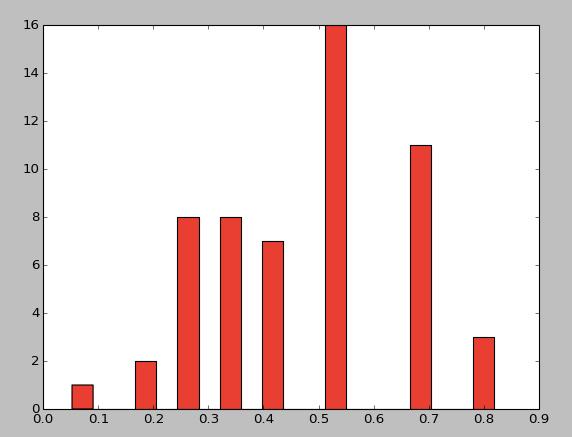
\includegraphics[scale = .4]{jaccard_sims}
\caption{Distribution of Jaccard Similarities}
\label{fig:jaccard_sims}
\end{figure}

\subsubsection{History-Sensitive Algorithm}

In \aref{fig:news_vis}, we have superimposed pictures from 
news articles that the tweets describe on a time axis, as
the hashtag referencing the article starts trending. 
We checked that the news was released (via Yahoo! News and Twitter)
at around the time our algorithm says the hashtag relating to the news
begins to trend. 

\begin{figure} 
\centering
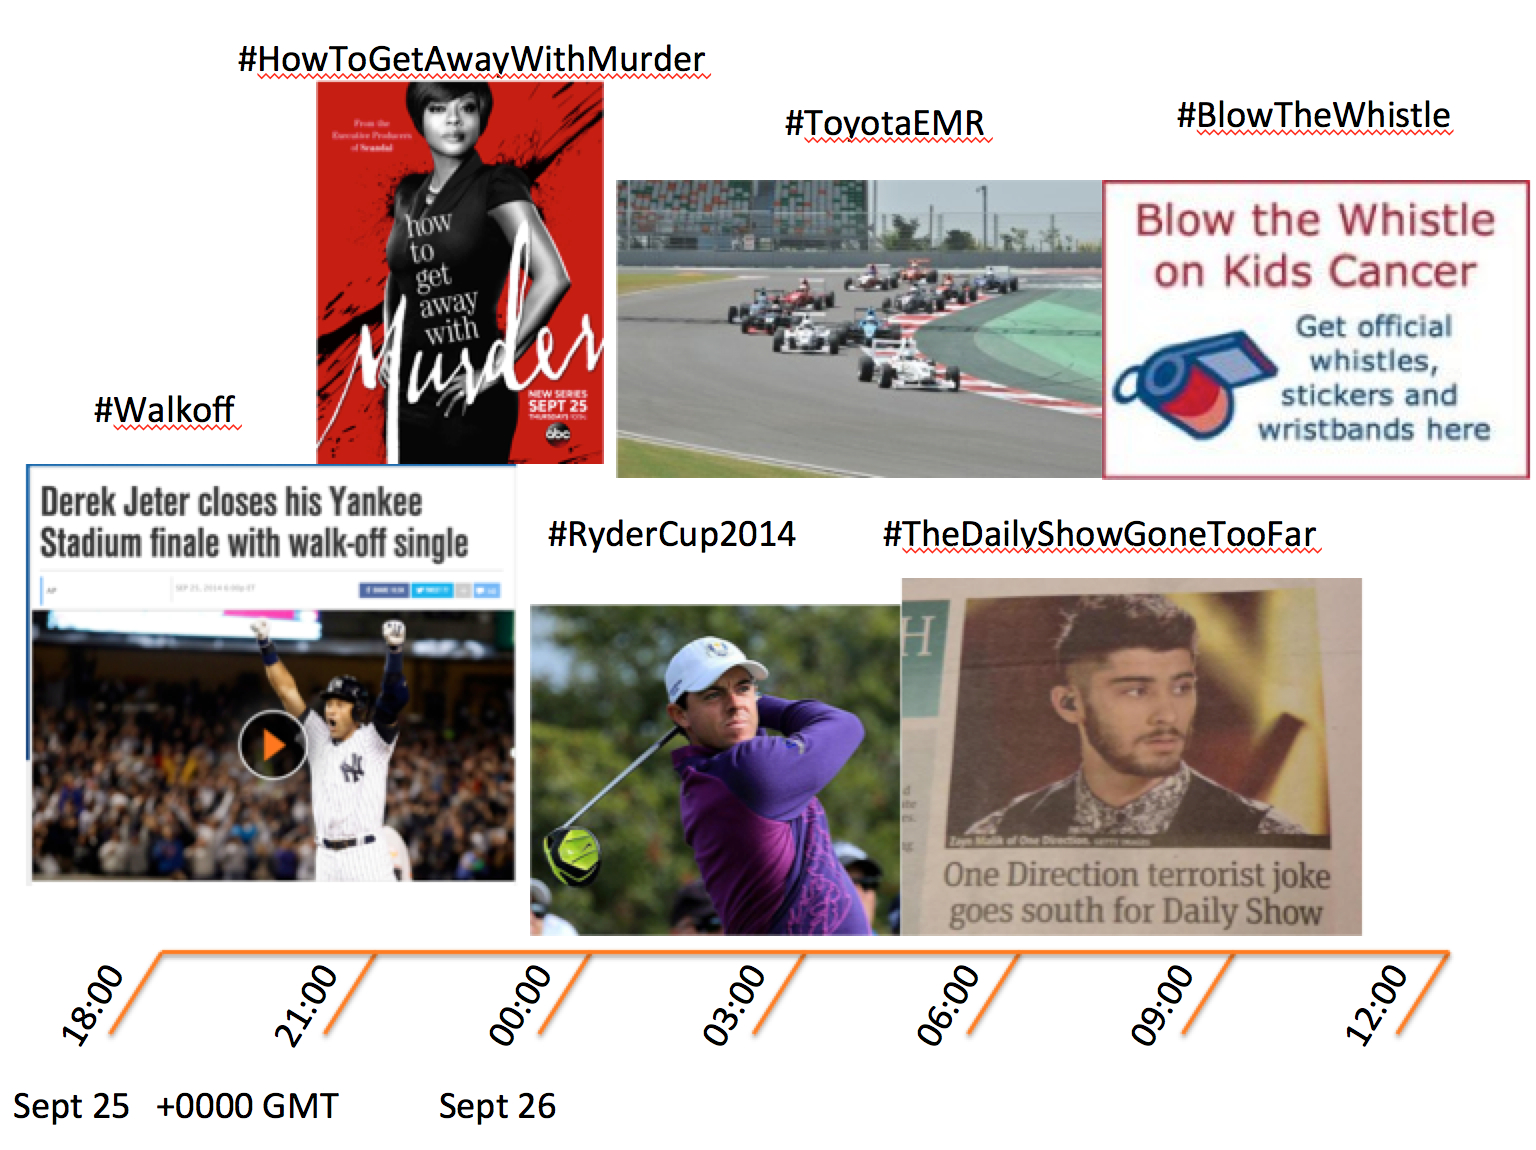
\includegraphics[scale = .4]{Timeline}
\caption{News Visualization of Trending Tweets}
\label{fig:news_vis}
\end{figure}

\subsubsection{Naive Algorithm}

We consider a few snapshots of duration $3$ hours each during
the last week of the month. 

%------------------------------------------------

\section{Discussion}

\subsection{Comparison of Naive and History-Sensitive Algorithms}


\subsection{Applicability to Real-Time Data}

do well to get month's worth of data in a few hours (2-3)

implementation wouldnt run in python, do it in C or something

for real data from firehose (all of it), we would use 
better infrastructure dedicated to processing all the data
would use parallel setup (this scheme is adaptable to parallel
setup)

seems reasonable if we have proper data storage setup.


%------------------------------------------------
\section{Future Work} \label{sec:Future Work}

With respect to the algorithms specifically, in the future we would want to adapt our approach to the history-sensitive algorithm and play with the parameters a bit more. We would also like to try different kernel functions to see how they performed. 

Then, we would like to try adapating our algorithms to real-time data: that is, hook up our algorithms to a significant portion of the Twitter firehose, after setting up the necessary hardware to process that amount of data. In order to aid with the processing, we would also ideally use a distributed system and parallelize
our code for better performance.

We also know that an estimation the top $k$ hashtags in a given time interval could provide a topic model for tweets. It could be interesting to use the top $k$ hashtags to build a time-sensitive topic model and analyze quantities including the speed of topic change, the variety of topics, and so on.

Even though not perhaps irrelevant to the specific task of identifying trending hashtags, 
the approach of the history-sensitive algorithm may be useful in other domains.
Future work could also investigate the performance of the history-sensitive algorithm on other data streams of interest, for instance, Wikipedia edits -- our goal would be to estimate which Wikipedia topics are being edited the most at any given time interval of some length. Another interesting application of this algorithm to test would be the real-time estimatation of the hottest selling stocks on Wall Street to see if either of these settings results in a significant improvement over the naive algorithm.

\section{Appendix I: Code and Visualizations} \label{sec:Appendix_code_viz}

We provide a link to \href{https://github.com/kiranvodrahalli/cos521/}{all our code}, as well as to an online hosting of the \href{http://www.princeton.edu/~awlee/trends.html}{frequency visualization}.

In our code, we made use of two libraries written by other people, which we modified. One of these was a Count-Min sketch implementation in Python, and another was a Fibonacci heap implementation, also in Python. These program files are in our codebase, with appropriate citations at the top of each document. Furthermore, we used multiple standard Python libraries in our code.

\section{Appendix II: Top-$k$ Hashtags in $6$ Interesting Time Chunks} \label{sec:Appendix_topk}

In [FIGURE WHATEVER] we present side-by-side the top $10$ hashtags in six $3$-hour intervals for both the naive algorithm and the history-sensitive algorithm, along with their heap priorities. Note that the heap priorities span
a fair range from $0$ to $1$, and are not clustered around $1$ or $0$, implying the algorithms are actually differentiating the hashtags as trending and not trending. To see all $56$ $3$-hour intervals for both algorithms, see our \href{https://github.com/kiranvodrahalli/cos521/}{Github}.

%----------------------------------------------------------------------------------------
%	REFERENCE LIST
%----------------------------------------------------------------------------------------

\begin{thebibliography}{99} % Bibliography - this is intentionally simple in this template


\bibitem[Burks2014]{Burks:2014}
Burks, L., Miller, M., and Zadeh, R. (2014). 
\newblock RAPID ESTIMATE OF GROUND SHAKING INTENSITY BY COMBINING SIMPLE EARTHQUAKE CHARACTERISTICS WITH TWEETS. 
\newblock {\em Tenth U.S. National Conference on Earthquake Engineering Frontiers of Earthquake Engineering}. Retrieved from \href{http://www.stanford.edu/~rezab/papers/eqtweets.pdf}{http://www.stanford.edu/~rezab/papers/eqtweets.pdf}

\bibitem[Cormode2005]{Cormode:2005}
Cormode, G., and Muthukrishnan, S. (2005). 
\newblock An improved data stream summary: The count-min sketch and its applications. 
\newblock {\em Journal of Algorithms, 55}(1), pp. 58-75.

\bibitem[MITNews2012]{MITNews2012}
Hardesty, Larry. 
\newblock {\em "Predicting What Topics Will Trend on Twitter."} 
\newblock MIT News Office. MIT, 1 Nov. 2012. Web. 13 Jan. 2015. \href{http://newsoffice.mit.edu/2012/predicting-twitter-trending-topics-1101}{http://newsoffice.mit.edu/2012/predicting-twitter-trending-topics-1101}.

\bibitem[Matusevych2012]{Matusevych:2012}
Matusevych, S., Smola, A., and Ahmed, A. (2012).
\newblock Hokusai--Sketching Streams in Real Time.
\newblock {\em UAI '12: 28th conference on Uncertainty in Artificial Intelligence}, pp. 594-603.

\bibitem[Twitter2014]{Twitter2014}
Twitter, Inc. (2014). 
\newblock {\em Archive Team JSON Download of Twitter Stream 2014-09}. 
\newblock Retrieved from \href{https://archive.org/details/twitterstream}{https://archive.org/details/twitterstream}.
 
\end{thebibliography}

%----------------------------------------------------------------------------------------



\end{document}
